% !TEX encoding = UTF-8 Unicode
\documentclass[a4paper]{article}


\usepackage[T1]{fontenc}     % För svenska bokstäver
\usepackage[utf8]{inputenc}  % Teckenkodning UTF8
\usepackage[swedish]{babel}  % För svensk avstavning och svenska
                             % rubriker (t ex "Innehållsförteckning")
\usepackage{fancyvrb}        % För programlistor med tabulatorer
\fvset{tabsize=4}            % Tabulatorpositioner
\fvset{fontsize=\small}      % Lagom storlek för programlistor

\title{Mandelbrot \\
	Inlämningsuppgift 2, Programmeringsteknik för C/D}
\author{Adam Hansson Lyrén, C11 (dic11aha@student.lu.se)\\
Johan Bäversjö, C11 (dic11jba@student.lu.se)}


% *** Tillägg för denna rapport. ***
% Paket:
\usepackage{graphicx}         % För att inkludera bilder.

% Kommandon i denna rapport
\newcommand{\code}[1]{\texttt{#1}} % För programkod i text.
% *** Slut på tillägg för denna rapport. ***


\begin{document}              % Början på dokumentet

\maketitle
\thispagestyle{empty}
\newpage
\setcounter{page}{1}
\section{Bakgrund}
Uppgiften består i att skapa en Mandelbrots-figur. Vi ska till en börjar skapa en klass som hanterar komplexa tal och därigenom skapa ett komplext talplan som i sin tur skall efter olika beräkningar, bilda Mandelbrotsfiguren. Vi har fått ett färdigt GUI att jobba med där vi behöver implementera lite olika funktioner som: zoomning, återställning av figuren och målning figuren.
\newline
Vi skall dessutom ge stöd till inställningar: med eller utan färg, upplösning och ett fält med extra inställningar som kan vara lite vad som helst.
\newline
\newline
Så här kommer en Mandelbrotsfigur att se ut helt utzoomad:
\begin{center}
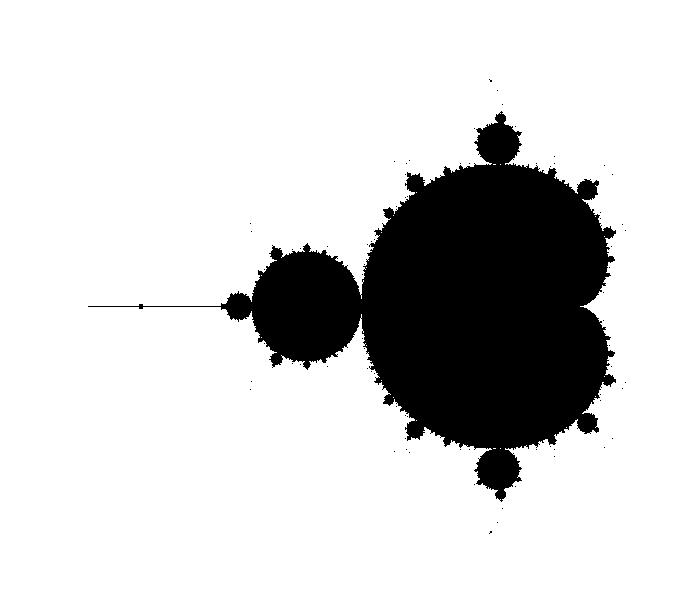
\includegraphics[scale=0.29]{mandelbrot_print_1.jpg}
\end{center}
 
\section{Modell}
Modellen av programmet innehåller följande klasser:


\begin{tabular}{lp{8cm}}
\code{Complex} & Klass som beskriver ett Komplext tal i planet \\
\code{TestComplex} & Klass som beskriver ett unit-test för klassen \code{Complex} \\
\code{Mandelbrot} & Innehåller \code{main} metoden som skapar det färdigställda GUI:t och hanterar kommandon \\
\code{Generator} & Innehåller ett antal metoder som genererar det komplexa talplanet och målar ut en figur beroende på om talet är inom Mandelbrots-mängden eller inte \\

\end{tabular}

\vspace{\baselineskip}
Nedan följer en beskrivning till flödet i programmet:

\begin{itemize}
\item Det färdiga GUI:t av typen \code{MandelbrotGUI} initialiseras och ritas ut i ett fönster.
\item I \code{Mandelbrot} klassens \code{main} metod körs en evig loop som väntar på innmatning från GUI:t; Render, Zoom, Reset och Quit.
\item Vid ett knapptryck på render-knappen så sker huvuddelen av programmet. Event-loopen i \code{main}-metoden når \code{MandelbrotGUI.RENDER} fallet (case) och där kallas \code{Generator}-klassens render metod. I denna metod kommer mandelbrotfiguren ritas.
\begin{itemize}
	\item I \code{Generator}-klassen genereras ett färgspektrum när klassen först laddas. Detta sker i ett \code{static} block eftersom det endast behöver ske en gång under programmets livstid. Vi genererar färgerna utifrån en palett som hårdkodad från början. \newline
	Färgerna i vårt färgspektrum genereras så att de går från första färgen i paletten till nästa färg. Vårt färgspektrum består av 255 färger och \code{render()} metoden kommer använda dessa beroende på hastigheten ett tal går utanför mandelbråtsmängden. Algoritmen för detta beskrivs i detalj i klassen \code{Generator}.
	\item I \code{render()}-metoden avaktiveras först GUI:t eftersom denna metod kan ta lång tid. I slutet av metoden aktiveras det igen. Efter detta hämtas värden för inställningar såsom upplösning, antal iterationer för mandelbrotalgoritmen och färginställningar.
	\item Nu kallas \code{mesh()}-metoden för att generera ett komplext talplan där värderna ändras successivt från minsta reella och största imaginära högst upp till vänster mot största reella och minsta imaginära längst ner till höger i det komplexa talplanet.
	\item Efter detta går programmet igenom samtliga komplexa tal och kollar ifall de är inom mandelbrotsmängden. För att detta programmet inte ska köras i all evighet bestämmer vi att ett komplex tal är inom mandelbrotsmängden ifall det komplexa talets absolutvärde divergerar med 2 eller fler längdenheter. Ifall ett tal är inom mandelbrotsmängden så får den en svart färg i figuren med samma koordinater. Annars tilldelas en vit eller färgad färg beroende på användarens inställningar.
\end{itemize}
\item Vid en inzoomning i bilden så körs endast \code{render()}-metoden på nytt. \code{MandelbrotGUI}:t hanterar inzoomning själv och vår \code{render()}-metod utnyttjar dessa värden.
\item Vid ett knapptryck på reset-knappen så återställs både inzoomning och figuren i det grafiska gränssnittet.
\item Vid ett knapptryck på quit-knappen så stängs programmet av med statuskoden 0 (Inga fel).
\end{itemize}

\section{Brister och kommentarer}
Istället för att användaren manuellt behöver specifiera antalet iterationer, som behövs göras vid mycket inzoomning hade programmet kunna sköta detta. Antalet iterationer skulle kunna vara en funktion av zoom nivån för att alltid ge en högupplöst bild.

De färger som används i färgläget hade användaren själv kunnat specifiera med en färgväljare i gränssnittet. Man hade kunnat välja ett obegränsat antal färger och se direkt hur de blandats i ett spektrum i GUI:t.

För att kunna koppla ihop det här programmet med andra system hade vi velat att programmet skulle ha ett CLI. Detta hade gjort det enkelt att koppla ihop vårt program med andra system. Programmet skulle kunna ta fokuspunkt, zoom och antal iterationer som inparametrar och en JPG bild som output. Detta hade varit ett enkelt tilläg till programmet då det koden inte behövs modifieras mycket. En ny GUI implementation som emulerar ett gui hade behövts skrivas, samt kod för att hantera input/output.

\begin{center}
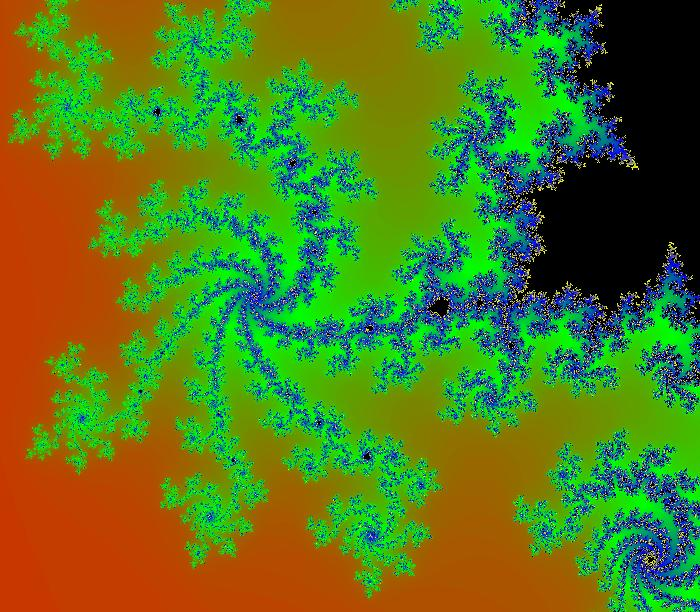
\includegraphics[scale=0.29]{mandelbrot_print_2.jpg}
\newline
Resolution: Very high, Mode: Color, Iterations: 200, Real axis: [-0.66,-0.64], Imaginary axis: [0.40, 0.42].
\newline
\newline
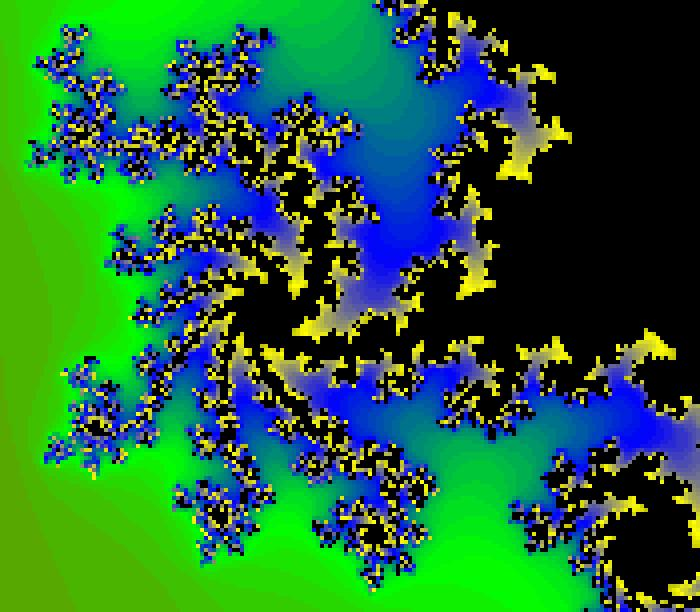
\includegraphics[scale=0.29]{mandelbrot_print_3.jpg}
\newline
Resolution: Medium, Mode: Color, Iterations: 70, Real axis: [-0.67,-0.64], Imaginary axis: [0.40, 0.43]. Ungefär samma område som föregående figur.
\end{center}

\section{Programlistor}
Klasserna finns i filer med motsvarande namn. Till exempel innehåller filen  \code{Generator.java} klassen \code{Generator}. Alla klasser som används finns i samma katalog som huvudprogrammet

\subsection{\code{Complex}}
\VerbatimInput{../src/Complex.java}

\subsection{\code{TestComplex}}
\VerbatimInput{../src/TestComplex.java}

\subsection{\code{Mandelbrot}}
\VerbatimInput{../src/Mandelbrot.java}

\subsection{\code{Generator}}
\VerbatimInput{../src/Generator.java}

\end{document}                  % Slut på dokumentet
